

\documentclass[11pt,a4paper,twoside]{book} % Use the UniMelb Dissertation Template
\usepackage{../manuscript/style/uomthesis}
% User defined commands

%%
%% Custom Hyphenations
%%
%%
\hyphenation{cross-talk au-di-tory adap-t-a-tion phe-nom-en-o-lo-g-i-cal
  syn-a-pse co-inc-id-ence Tub-er-culo-vent-ral glyc-in-ergic psycho-phys-ical
  asym-met-ric ex-plor-at-ory pot-as-sium op-ti-mi-sa-tion au-di-t-ory system
  Neuro-in-for-mat-ics mar-g-in-al par-a-m-eters Rh-ode Neu-ro-fit-ter
  elec-tro-phys-io-log-i-cal in-fer-ring the con-nec-tiv-i-ty with-in
  non-lin-ear ap-pr-oa-ch-es stel-late mi-cro-cir-cuit show-ing synap-tic
  in-ter-ac-tion iso-lam-inar pop-u-la-tion evo-l-ved com-part-ment
  con-duc-tance mod-els Hod-g-kin Hux-l-ey gluta-m-at-er-gic gen-o-mes
  Theu-nis-sen re-sp-on-se co-inc-id-ence det-e-ctor exp-eri-men-tal
  ac-cu-mu-lated neu-ro-science cre-ate de-tailed ex-ten-sively stud-ied
  In-tra-cel-lu-lar neur-rons in-tra-cel-lu-lar in-ves-ti-ga-tion se-quen-tial
  de-ter-min-ed cat-e-gor-is-ed im-me-di-ate sen-si-tiv-ity bicu-cu-line
  mul-ti-ple in-hib-it-ory com-mis-sural path-way re-cip-ro-cal fre-quency
  po-si-tion func-tion de-lay prep-a-ra-tions iso-lated oct-o-pus in-sen-si-tive
  Chop-per im-preg-na-tion phys-i-o-log-i-cal ef-fect GABA-er-gic in-puts on-set
  chop-pers pri-mar-ily  gen-er-ate ar-ray gaus-sian ran-dom num-bers
  in-ves-ti-gat-ing im-p-or-tant phys-i-o-log-i-cal mech-a-nisms}
%%
%% Sample custom-configuration
%%
%%   You are encouraged to modify the following section with any of your
%%   own custom commands, packages, etc.
%%

%error 'You should modify this section and remove this error.'

% for URLs
\usepackage{url}

% AMS packages
%\usepackage{amsfonts}
\usepackage{amssymb}
\usepackage[fleqn]{amsmath}   % displayed equations flush left
%\setlength{\mathindent}{0em}
%\usepackage{amsthm}
\usepackage[mathscr]{eucal}

\newcommand{\vect}[1]{\mathbf{#1}}


% Allow equations to break over pages...
\interdisplaylinepenalty=2500
% Command to stop equation breaks
% Note: enclose this in braces when used...
\newcommand{\donotsplitoverpages}{\interdisplaylinepenalty=10000}

%% Graphics
% \ifx\pdftexversion\undefined
%  \usepackage[dvips]{graphicx}
% \else
%  \usepackage[pdftex]{graphicx}
% \fi

%% My Graphics and Hyperlinks stuff
\usepackage{ifpdf}
 \ifpdf
   \pdfoutput=1
   \usepackage[pdftex]{graphicx}  % uncomment if using graphicx
\usepackage[final,          % override "draft" which means "do nothing"
            colorlinks,     % rather than outlining them in boxes
            linkcolor=black, % override truly awful colour choices
            citecolor=black, %   (ditto)
            urlcolor=black,  %   (ditto)
            ]{hyperref}

 \ifx\pdfoutput\undefined \usepackage[ps2pdf,
 bookmarks=true,
 bookmarksnumbered=true,
 breaklinks=true,
            final,          % override "draft" which means "do nothing"
            colorlinks,     % rather than outlining them in boxes
            linkcolor=black, % override truly awful colour choices
            citecolor=black, %   (ditto)
            urlcolor=black,  %   (ditto)
            ]{hyperref}

% \usepackage[pdftex]{hyperref}  % uncomment if using hyperref
%  \usepackage[ps2pdf]{thumbpdf}
 \DeclareGraphicsExtensions{.eps,.bmp}
  \else
 \DeclareGraphicsExtensions{.png,.pdf,.jpg,.JPEG}
  \usepackage{epstopdf}
 %\usepackage[pdftex,bookmarks=true,bookmarksnumbered=true,breaklinks=true]{hyperref}
  \pdfadjustspacing=1
  \usepackage[pdftex]{thumbpdf}
  \fi
 \else
   \usepackage[dvips]{graphicx}  % uncomment if using graphicx
    % comment if not using hyperref
 \usepackage[final,          % override "draft" which means "do nothing"
            colorlinks,     % rather than outlining them in boxes
            linkcolor=black, % override truly awful colour choices
            citecolor=black, %   (ditto)
            urlcolor=black,  %   (ditto)
             ]{hyperref}
 \DeclareGraphicsExtensions{.eps,.bmp}
\fi
% Enable IEEE macros
%\usepackage{IEEEtrantools}

% Use a plain bibliography style
%\bibliographystyle{plain}
% Use the IEEE bibliography style (sorted)
%\bibliographystyle{IEEEtrans}
% Use the IEEE bibliography style (unsorted; order of reference)
%\bibliographystyle{IEEEtran}

% For isolated bibliographies
\usepackage{bibunits}

\usepackage{color}
%\usepackage[noadjust]{cite}
\usepackage{caption}
\usepackage{breakurl} % necessary to break URLs when using LaTeX-> dvips -> Ps2PDF, must be after hyperref

% For cool tables
\usepackage{array}
\usepackage{tabularx}  % automatically adjusts column width in tables
\usepackage{multirow}  % allows entries spanning several rows
\usepackage{colortbl}  % allows coloring tables


% For algorithms
%\usepackage{algorithm}
%\usepackage{algorithmic}

% For cases
\usepackage{sublabel}

% For theroem numbers having the chapter included
%\usepackage{style/chngcntr}

% For cool theorem styles
%\usepackage[amsthm]{ntheorem}
%%\theorembodyfont{\normalfont}
%
%% Theorem definition
%\newtheorem{theorem}{Theorem}
%\counterwithin{theorem}{chapter}
%
%% Corollary definition
%\newtheorem{corollary}{Corollary}
%\counterwithin{corollary}{chapter}
%
%% Result definition
%\newtheorem{result}{Result}
%\counterwithin{result}{chapter}
%
%% Lemma definition
%\newtheorem{lemma}{Lemma}
%\counterwithin{lemma}{chapter}
%
%% Proposition definition
%\newtheorem{proposition}{Proposition}
%\counterwithin{proposition}{chapter}
%
%% Definition definition!
%\newtheorem{definition}{Definition}
%\counterwithin{definition}{chapter}
%
%% Remark definition (no counter?)
%\newenvironment{remark}{\emph{Remark:~}}{}
%
%% Fact definition (no counter?)
%\newenvironment{fact}{\emph{Fact:~}}{}

% (Re)Set the figure path
\newcommand{\setfigurepath}[1]{%
\ifx\figurepath\undefined
	\newcommand{\figurepath}{#1}
\else
	\renewcommand{\figurepath}{#1}
\fi%
}

% Used in the continued list environment below
\newcounter{continuedlist}

% Continued list environment
\newenvironment{continuedlist}{%
	\begin{enumerate}%
		% Space out each item
		\setlength{\itemsep}{1.25em}%
		% Start the enumeration from the previous value
		\setcounter{enumi}{\value{continuedlist}} %
}{ %
  % Save the counter to continue it later
  \setcounter{continuedlist}{\value{enumi}}%
  \end{enumerate}%
  % \vspace{1.25em}% 
  \vspace{1em}%
}

% Spaced out list environment
\newenvironment{spacedoutlist}{%
	\begin{itemize}%
		% Space out each item
		\setlength{\itemsep}{1.25em}%
}{\end{itemize}}


%% My added packages


\usepackage[usenames,dvipsnames]{xcolor}
\definecolor{halfgray}{gray}{0.55}

\usepackage{listings}
\lstset{language=C++,%[LaTeX]Tex,%
    keywordstyle=\color{RoyalBlue},%\bfseries,
    basicstyle=\small\sffamily,
    identifierstyle=\color{NavyBlue},
    commentstyle=\color{Green}\rmfamily,
    stringstyle=\sffamily,
    numbers=left,%none,%
    numberstyle=\scriptsize,%\tiny
    stepnumber=5,
    numbersep=8pt,
    showstringspaces=false,
    breaklines=true,
    %frameround=ftff,
    %frame=single
    %frame=L
    lineskip=-5pt
}


% \lstset{language=Octave,                % choose the language of the code
% basicstyle=\footnotesize,       % the size of the fonts that are used for the code
% numbers=left,                   % where to put the line-numbers
% numberstyle=\footnotesize,      % the size of the fonts that are used for the line-numbers
% stepnumber=2,                   % the step between two line-numbers. If it's 1 each line will be numbered
% numbersep=5pt,                  % how far the line-numbers are from the code
% backgroundcolor=\color{white},  % choose the background color. You must add \usepackage{color}
% showspaces=false,               % show spaces adding particular underscores
% showstringspaces=false,         % underline spaces within strings
% showtabs=false,                 % show tabs within strings adding particular underscores
% frame=single,			% adds a frame around the code
% tabsize=2,			% sets default tabsize to 2 spaces
% captionpos=b,			% sets the caption-position to bottom
% breaklines=true,		% sets automatic line breaking
% breakatwhitespace=false,	% sets if automatic breaks should only happen at whitespace
% lineskip=-5pt  %
% }

\ifx\setcitestyle\undefined
\usepackage[sort,round,authoryear]{natbib}
\setcitestyle{aysep={}} % J Neurophys formatting
\fi

\usepackage{xspace}
\usepackage{rotating}
\usepackage{tikz}
\usepackage{calc}

\newcommand{\hdr}[3]{%
\multicolumn{#1}{|l|}{\color{white}\cellcolor[gray]{0.0}%
\textbf{\makebox[0.05\linewidth][l]{#2}\hspace{0.45\linewidth}\makebox[0pt][c]{#3}}%
%\textbf{\makebox[0pt]{#2}\hspace{0.5\linewidth}\makebox[0pt][c]{#3}}%
}}
 % Nordelie table environment
\newenvironment{ntab}[4]{
\noindent\begin{tabularx}{\linewidth}{#1}\hline 
\multicolumn{#2}{|l|}{\color{white}\cellcolor[gray]{0.0}\textbf{#3\hfill{}{#4}\hfill{}}}
}{
\end{tabularx}
\vspace{1ex}
}



\usepackage[colorinlistoftodos,backgroundcolor=yellow!35,textsize=footnotesize]{todonotes}
\newcommand{\yellownote}[1]{\todo[inline]{#1}}


\usepackage{scrtime}
%\usepackage{mparhack}

%\setlength{\parskip}{0ex} or {1.2ex}
%\setlength{\parindent}{0em} or {0ex}

\usepackage[australian]{babel}

\usepackage{booktabs,ltxtable,ctable,dcolumn}
\newcommand{\otoprule}{\midrule[\heavyrulewidth]}

\usepackage{doipubmed}

% For subfigures
\usepackage{keyval}
\usepackage[config,labelfont={sf,bf}]{subfig}
%\captionsetup[table]{position=top}
%\captionsetup[subtable]{position=top}
%\usepackage[heightadjust=all,valign=t]{floatrow}
%\usepackage{fr-subfig}
%\floatsetup{style=Plaintop}
%\usepackage{subfigure}

\usepackage{lscape}

\newcommand{\code}[1]{\mbox{\normalfont\texttt{#1}}}
\newcommand{\progname}[1]{\mbox{\normalfont\textsf{#1}}}
\newcommand{\figfont}[1]{\large{\textbf{\textsf{#1}}}}

% User defined commands

%\usepackage{pstricks}

%\newenvironment{etabular}[1]{
%\noindent\begin{tabularx}{\linewidth}{#1}\hline %    \hdr{#2}{#3}{#4}\\ \hline
%}{\end{tabularx} \vspace{2ex}}

\usepackage{xspace}
%% Glossary

% ANF to Golgi
\newcommand{\ANFGLG}{\protect\ensuremath{\mbox{ANF} \to \mbox{GLG}\xspace}}
\newcommand{\HSRGLG}{\protect\ensuremath{\mbox{HSR} \to \mbox{GLG}\xspace}}
\newcommand{\LSRGLG}{\protect\ensuremath{\mbox{LSR} \to \mbox{GLG}\xspace}}
\newcommand{\wANFGLG}{\protect\ensuremath{w_{\ANFGLG}\xspace}}
\newcommand{\wLSRGLG}{\protect\ensuremath{w_{\LSRGLG}\xspace}}
\newcommand{\wHSRGLG}{\protect\ensuremath{w_{\HSRGLG}\xspace}}
\newcommand{\nLSRGLG}{\protect\ensuremath{n_{\LSRGLG}\xspace}}
\newcommand{\nHSRGLG}{\protect\ensuremath{n_{\HSRGLG}\xspace}}
\newcommand{\sANFGLG}{\protect\ensuremath{s_{\ANFGLG}\xspace}}
\newcommand{\sLSRGLG}{\protect\ensuremath{s_{\LSRGLG}\xspace}}
\newcommand{\sHSRGLG}{\protect\ensuremath{s_{\HSRGLG}\xspace}}
\newcommand{\dANFGLG}{\protect\ensuremath{d_{\ANFGLG}\xspace}}

%ANF to D-stellate
\newcommand{\ANFDS}{\protect\ensuremath{\mbox{ANF} \to \mbox{DS}\xspace}}
\newcommand{\HSRDS}{\protect\ensuremath{\mbox{HSR} \to \mbox{DS}\xspace}}
\newcommand{\LSRDS}{\protect\ensuremath{\mbox{LSR} \to \mbox{DS}\xspace}}
\newcommand{\wANFDS}{\ensuremath{w_{\ANFDS}\xspace}}
\newcommand{\wLSRDS}{\protect\ensuremath{w_{\LSRDS}\xspace}}
\newcommand{\wHSRDS}{\protect\ensuremath{w_{\HSRDS}\xspace}}
\newcommand{\nLSRDS}{\protect\ensuremath{n_{\LSRDS}\xspace}}
\newcommand{\nHSRDS}{\protect\ensuremath{n_{\HSRDS}\xspace}}
\newcommand{\dANFDS}{\protect\ensuremath{d_{\ANFDS}\xspace}}
\newcommand{\sANFDSh}{\protect\ensuremath{s^+_{\ANFDS}\xspace}}
\newcommand{\sANFDSl}{\protect\ensuremath{s^-_{\ANFDS}\xspace}}

%ANF to T-stellate
\newcommand{\ANFTS}{\protect\ensuremath{\mbox{ANF} \to \mbox{TS}\xspace}}
\newcommand{\HSRTS}{\protect\ensuremath{\mbox{HSR} \to \mbox{TS}\xspace}}
\newcommand{\LSRTS}{\protect\ensuremath{\mbox{LSR} \to \mbox{TS}\xspace}}
\newcommand{\wANFTS}{\protect\ensuremath{w_{\ANFTS}\xspace}}
\newcommand{\nLSRTS}{\protect\ensuremath{n_{\LSRTS}\xspace}}
\newcommand{\nHSRTS}{\protect\ensuremath{n_{\HSRTS}\xspace}}
\newcommand{\sANFTS}{\protect\ensuremath{s_{\ANFTS}\xspace}}
\newcommand{\dANFTS}{\protect\ensuremath{d_{\ANFTS}\xspace}}

%ANF to Tuberculoventral
\newcommand{\ANFTV}{\ensuremath{\mbox{ANF} \to \mbox{TV}\xspace}}
\newcommand{\HSRTV}{\ensuremath{\mbox{HSR} \to \mbox{TV}\xspace}}
\newcommand{\LSRTV}{\ensuremath{\mbox{LSR} \to \mbox{TV}\xspace}}
\newcommand{\wANFTV}{\ensuremath{w_{\ANFTV}\xspace}}
\newcommand{\nLSRTV}{\ensuremath{n_{\LSRTV}\xspace}}
\newcommand{\nHSRTV}{\ensuremath{n_{\HSRTV}\xspace}}
\newcommand{\sANFTV}{\ensuremath{s_{\ANFTV}\xspace}}
\newcommand{\dANFTV}{\ensuremath{d_{\ANFTV}\xspace}}

%GLG to T-stellate
\newcommand{\GLGTS}{\protect\ensuremath{\mbox{GLG} \to \mbox{TS}\xspace}}
\newcommand{\wGLGTS}{\protect\ensuremath{w_{\GLGTS}\xspace}}
\newcommand{\nGLGTS}{\protect\ensuremath{n_{\GLGTS}\xspace}}
\newcommand{\sGLGTS}{\protect\ensuremath{s_{\GLGTS}\xspace}}
\newcommand{\dGLGTS}{\protect\ensuremath{d_{\GLGTS}\xspace}}
%GLG to D-stellate
\newcommand{\GLGDS}{\protect\ensuremath{\mbox{GLG} \to \mbox{DS}\xspace}}
\newcommand{\wGLGDS}{\protect\ensuremath{w_{\GLGDS}\xspace}}
\newcommand{\nGLGDS}{\protect\ensuremath{n_{\GLGDS}\xspace}}
\newcommand{\sGLGDS}{\protect\ensuremath{s_{\GLGDS}\xspace}}
\newcommand{\dGLGDS}{\protect\ensuremath{d_{\GLGDS}\xspace}}

% % TS to Golgi
% \newcommand{\GLGTS}{\protect\ensuremath{\mbox{GLG} \to \mbox{TS}\xspace}}
% \newcommand{\wTSGLG}{\protect\ensuremath{w_{}}\xspace}}
% \newcommand{\nTSGLG}{\protect\ensuremath{n_{\mbox{TS} \to \mbox{GLG}}\xspace}}
% \newcommand{\sTSGLG}{\protect\ensuremath{s_{\mbox{TS} \to \mbox{GLG}}\xspace}}
% \newcommand{\dTSGLG}{\protect\ensuremath{d_{\mbox{TS} \to \mbox{GLG}}\xspace}}

%TS to D-stellate
\newcommand{\TSDS}{\protect\ensuremath{\mbox{TS} \to \mbox{DS}\xspace}}
\newcommand{\wTSDS}{\protect\ensuremath{w_{\TSDS}\xspace}}
\newcommand{\nTSDS}{\protect\ensuremath{n_{\TSDS}\xspace}}
\newcommand{\sTSDS}{\protect\ensuremath{s_{\TSDS}\xspace}}
\newcommand{\dTSDS}{\protect\ensuremath{d_{\TSDS}\xspace}}
%TS to T-stellate
\newcommand{\TSTS}{\protect\ensuremath{\mbox{TS} \to \mbox{TS}\xspace}}
\newcommand{\wTSTS}{\protect\ensuremath{w_{\TSTS}\xspace}}
\newcommand{\nTSTS}{\protect\ensuremath{n_{\TSTS}\xspace}}
\newcommand{\sTSTS}{\protect\ensuremath{s_{\TSTS}\xspace}}
\newcommand{\dTSTS}{\protect\ensuremath{d_{\TSTS}\xspace}}

%TS to Tuberculoventral
\newcommand{\TSTV}{\protect\ensuremath{\mbox{TS} \to \mbox{TV}\xspace}}
\newcommand{\wTSTV}{\protect\ensuremath{w_{\TSTV}\xspace}}
\newcommand{\nTSTV}{\protect\ensuremath{n_{\TSTV}\xspace}}
\newcommand{\sTSTV}{\protect\ensuremath{s_{\TSTV}\xspace}}
\newcommand{\dTSTV}{\protect\ensuremath{d_{\TSTV}\xspace}}

% DS to Golgi
\newcommand{\DSGLG}{\protect\ensuremath{\mbox{DS} \to \mbox{GLG}\xspace}}
\newcommand{\wDSGLG}{\protect\ensuremath{w_{\DSGLG}\xspace}}
\newcommand{\nDSGLG}{\protect\ensuremath{n_{\DSGLG}\xspace}}
\newcommand{\sDSGLG}{\protect\ensuremath{s_{\DSGLG}\xspace}}
\newcommand{\dDSGLG}{\protect\ensuremath{d_{\DSGLG}\xspace}}

% %DS to D-stellate
% \newcommand{\DSDS}{\protect\ensuremath{\mbox{DS} \to \mbox{DS}\xspace}}
% \newcommand{\wDSDS}{\protect\ensuremath{w_{\DSDS}\xspace}}
% \newcommand{\nDSDS}{\protect\ensuremath{n_{\DSDS}\xspace}}
% \newcommand{\sDSDS}{\protect\ensuremath{s_{\DSDS}\xspace}}
% \newcommand{\dDSDS}{\protect\ensuremath{d_{\DSDS}\xspace}}

%DS to T-stellate
\newcommand{\DSTS}{\protect\ensuremath{\mbox{DS} \to \mbox{TS}\xspace}}
\newcommand{\wDSTS}{\protect\ensuremath{w_{\DSTS}\xspace}}
\newcommand{\nDSTS}{\protect\ensuremath{n_{\DSTS}\xspace}}
\newcommand{\sDSTS}{\protect\ensuremath{s_{\DSTS}\xspace}}
\newcommand{\dDSTS}{\protect\ensuremath{d_{\DSTS}\xspace}}

%DS to Tuberculoventral
\newcommand{\DSTV}{\protect\ensuremath{\mbox{DS} \to \mbox{TS}\xspace}}
\newcommand{\wDSTV}{\protect\ensuremath{w_{\DSTV}\xspace}}
\newcommand{\nDSTV}{\protect\ensuremath{n_{\DSTV}\xspace}}
\newcommand{\sDSTV}{\protect\ensuremath{s_{\DSTV}\xspace}}
\newcommand{\dDSTV}{\protect\ensuremath{d_{\DSTV}\xspace}}
\newcommand{\oDSTV}{\protect\ensuremath{o_{\DSTV}\xspace}}

% TV to Golgi
\newcommand{\TVGLG}{\protect\ensuremath{\mbox{TV} \to \mbox{GLG}\xspace}}
\newcommand{\wTVGLG}{\protect\ensuremath{w_{\TVGLG}\xspace}}
\newcommand{\nTVGLG}{\protect\ensuremath{n_{\TVGLG}\xspace}}
\newcommand{\sTVGLG}{\protect\ensuremath{s_{\TVGLG}\xspace}}
\newcommand{\dTVGLG}{\protect\ensuremath{d_{\TVGLG}\xspace}}

%TV to D-stellate
\newcommand{\TVDS}{\protect\ensuremath{\mbox{TV} \to \mbox{DS}\xspace}}
\newcommand{\wTVDS}{\protect\ensuremath{w_{\TVDS}\xspace}}
\newcommand{\nTVDS}{\protect\ensuremath{n_{\TVDS}\xspace}}
\newcommand{\sTVDS}{\protect\ensuremath{s_{\TVDS}\xspace}}
\newcommand{\dTVDS}{\protect\ensuremath{d_{\TVDS}\xspace}}

%TV to T-stellate
\newcommand{\TVTS}{\protect\ensuremath{\mbox{TV} \to \mbox{TS}\xspace}}
\newcommand{\wTVTS}{\protect\ensuremath{w_{\TVTS}\xspace}}
\newcommand{\nTVTS}{\protect\ensuremath{n_{\TVTS}\xspace}}
\newcommand{\sTVTS}{\protect\ensuremath{s_{\TVTS}\xspace}}
\newcommand{\dTVTS}{\protect\ensuremath{d_{\TVTS}\xspace}}

%TV to Tuberculoventral
\newcommand{\TVTV}{\protect\ensuremath{\mbox{TV} \to \mbox{TV}\xspace}}
\newcommand{\wTVTV}{\protect\ensuremath{w_{\TVTV}\xspace}}
\newcommand{\nTVTV}{\protect\ensuremath{n_{\TVTV}\xspace}}
\newcommand{\sTVTV}{\protect\ensuremath{s_{\TVTV}\xspace}}
\newcommand{\dTVTV}{\protect\ensuremath{d_{\TVTV}\xspace}}


%Other common symbols
\newcommand{\GABAa}{\ensuremath{\mbox{GABA}_\mbox{A}}}


\graphicspath{{../../soma/netmod/cnstellate/golgi/}{../../soma/netmod/cnstellate/}}
\begin{document}

%%%%%%%%%%%%%%%%%%%%%%%%%%%%%%%%%%%%%%%%%%%%%%%%%%%%%%





%%%%%%%%%%%%%%%%%%%%%%%%%%%%%%%%%%%%%%%%%%%%%
\graphicspath{{/media/data/Work/cnstellate/golgi/}{/media/data/Work/Responses/}{/media/data/Work/cnstellate/Responses/}{../figures/}{./gfx/}}
%%%%%%%%%%%%%%%%%%%%%%%%%%%%%%%%%%%%%%%%%%%%%

\section[Golgi Cell Model]{Golgi Cell Model: Optimisation using
  monotonic rate-level responses in marginal shell units}
\label{sec:golgi-cell-model}
% Modelling in the auditory periphery has benefited extensively from
% the work of Liberman, Greewood, Patterson, Young, Sachs and others,
% in acoustic \texttt{in vivo} experiments.

\subsection{Background}

The source of GABAergic inputs to cells in the mammalian CN is
somewhat contentious. Despite studies showing that GABAergic inputs to
the CN generally arise in the peri-olivary regions of the medulla in
cats \citep{OstapoffBensonEtAl:1997} and birds
\citep{LachicaRubsamenEtAl:1995,YangMonsivaisEtAl:1999}, slice
preparations of the isolated murine VCN have shown sensitivity to
bicuculine in TS and DS cells \citep{FerragamoGoldingEtAl:1998a}.  The
only known source of GABA intrinsic to the VCN are the golgi cells of
the granule cell domain (GCD) overlying the VCN 
\citep[Fig.~\ref{fig:CNdiagram}]{Mugnaini:1985,FerragamoGoldingEtAl:1998}.
The presence of GABAergic inputs to TS, DS and TV cells has been
verified by labeled terminals adjacent to the soma and dendrites
\citep{SmithRhode:1989,AwatramaniTurecekEtAl:2005,BabalianRyugoEtAl:2003}
and release from inhibition in their response areas with
ionotopopheretic application of the \GABA antagonist, bicuculine
\citep{EvansZhao:1998,CasparyBackoffEtAl:1994,BackoffShadduckEtAl:1999,FerragamoGoldingEtAl:1998a}.

\medskip{}

Other studies in the rat cochlear nucleus relating to the Golgi cell or GABA:
\begin{itemize}
\item \citep{MugnainiOsenEtAl:1980} Fine structure of granule cells
  and related interneurons (termed {Golgi} cells) in the cochlear
  nuclear complex of cat, rat and mouse
\item GABAa expression in the rat brainstem  \citep{CamposCaboEtAl:2001}
\item \citep{Alibardi:2003a} Ultrastructural distribution of
  glycinergic and {{GABAergic}} neurons and axon terminals in the rat
  dorsal cochlear nucleus, with emphasis on granule cell areas
\item \citep{AwatramaniTurecekEtAl:2005} Staggered {Development} of
  {GABAergic} and {Glycinergic} {Transmission} in the {MNTB}
\end{itemize}

\medskip{}

Role of GABA in the VCN
\begin{itemize}
\item Effects of microiontophoretically applied glycine and {GABA} on
  neuronal response patterns in the cochlear nuclei
  \citep{CasparyHaveyEtAl:1979}
\end{itemize}

\citep{Alibardi:2003a} rat CN complex -> Golgi-stellate cells
(fusiform layer: 2) in DCN contact granule and unipolar brush cells


\medskip{}

Inputs to golgi cells are more complicated than VCN cells in the core
regions. Golgi cells are sparse in the GCD, surrounded by the many,
smaller excitatory granule cells, that form small en passant
endings. Type II ANFs create diffuse glutamatergic release sites in
the GCD \citep{HurdHutsonEtAl:1999,BensonBrown:2004} that may
stimulate NMDA glutamate receptors in golgi cells
\citep{FerragamoGoldingEtAl:1998a}.

\medskip{}

Extracellular recordings from the GCD by \citet{GhoshalKim:1997}, are most likely from golgi
cells since granule cell somata are less than  $10 \mu m$ and very
narrow axons. The majority of recorded
units showed a monotonic increase in firing rate with increasing sound
intensity \citep{GhoshalKim:1997}. 


\medskip{}

The lack of extensive experimental data meant that a phenomenological model
would be preferred over the Hogkin-Huxley type neural model. A number of steps
were taken to investigate the golgi cell model.

\medskip{}

The known GABAergic input to VCN units comes primarily from the superior olive
(ref), but the presence of active GABA synapses in isolated VCN slices by
\citet{FerragamoGoldingEtAl:1998} led to further investigation of
golgi cells in the granule cell domain. \citet{FerragamoGoldingEtAl:1998a}
showed that golgi cells have a classic type-I current
response, which suggest they integrate inputs, and their response to
AN shocks were delayed by approximately 0.7~ms relative to the core
VCN units .  Ghosal and Kim
\citet{GhoshalKim:1997} examined the VCN marginal shell in cats (equivalent to the
GCD in mice) that golgi cells provide some sort of
automatic gain control to the principle VCN units, through their monotonic
responses to tones and noise.

\medskip{}

% (Reference) showed that in adult animals high-spontaneous rate ANFs do not
% project to the GCD; they do show that low-spontaneous rate ANFs do project into
% the GCD, albeit more profusely than in the core on the VCN.
   

\begin{figure}[htb]
  \centering
\resizebox{0.8\textwidth}{!}{\includegraphics{NoFigure}}
%  \resizebox{0.8\textwidth}{!}{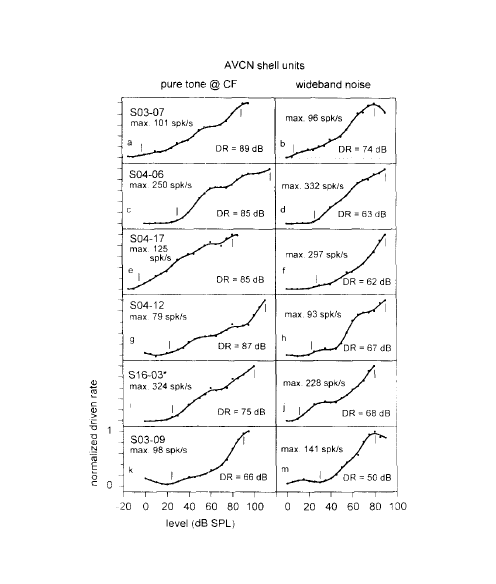
\includegraphics{GhoshalKim}}
\caption{Rate level response of unit S03-07 (CF 21~kHz) from Fig2
  \citep{GhoshalKim:1997} }
\end{figure}




\newpage
\subsection{Implementation}

In the creation of the golgi cell model, we can reduce the explicit
responses of Golgi cells down to three major details: a) golgi cells are integrators due to their type-I~current clamp response, b) golgi cells are (most likely) monotonic to tone and noise rate increases, and
c) they have a significant delay of first spike latency relative to the core VCN units.


In Chapter~\ref{sec:GAChapter} and previous publications \citep{EagerGraydenEtAl:2006a}, the golgi cell model was implemented as a single-compartment conductance  neuron. Due to the unavailability of sufficient data regarding \emph{in vivo}
golgi cell responses, we have decided to simulate the response of
golgi cells using inputs from the auditory model's instantaneous rate outputs rather
than simulating the neural membrane. 


The instantaneous rate vector of a golgi cell model at CF channel
\emph{i} is created by :
\begin{itemize}
 \item a selection of ANF input channels centred at \emph{i} with a
 spread, \sLSRGLG;
 \item the instantaneous rate vectors of the LSR ANF's in each channel
 are weighted (with a gaussian function (mean=\emph{i},
 s.d.=$\sqrt{\sLSRGLG}$) and the weighted vectors are averaged; and
 \item the weighted average vector is convolved with an alpha function
 of time constant 5, to simulate the synaptic and membrane dynamics of
 golgi cells
\end{itemize}

\medskip{}

\yellowbox{this needs to be removed}
[NEURON code methods] Each golgi cell template consists of a spike generator, \emph{s}, and vector
objects representing the instantaneous rate, the spike times and
accumulated  spike times of the golgi cell. Parameters identifying
each cell include the \emph{channel} number, CF and bandwidth of ANF
input (actually the variance of the weight each auditory filter
channel contributes to the firing of the cell).


\vspace{1ex}
% - A ------------------------------------------------------------------------



Monotonic rate-level data from GCD in VCN \citep{GhoshalKim:1996} unit
S03-07 (CF 21~kHz) was used to optimise parameters ${\rm
golgi\_spon}$, \wLSRGLG, \wHSRGLG, and \sANFGLG\@.  The optimisation
method was a default using the principle-axis method.
\medskip{}


Due to its replication of granule cells in the model, weight for LSR \wLSRGLG and HSR \wHSRGLG are determined for all synapses, number \nLSRDS and \nHSRDS, delay \dANFGLG added to smoothing function to ensure conductance and dendritic filtering are included.

\subsubsection{Key design factors}
 - Choosing neural model: HH-type or Poisson
 - Problem of monotonic excitation at low level
  - added HSR to model to avoid added computation of MSR
 - Spread of ANF to GCD ARE broader than core VCN
  - are we spoiling the broth too early? 


\begin{figure}[hp!]
  \centering
  \includegraphics[width=0.9\textwidth,trim=0 110mm 1 55mm]{gfx/GolgiDiagram}
  \caption{ The golgi instantaneous-rate profile was generated using ANF
    profiles. $\mu$ and $\sigma$ control the spread of connections
    across frequency channels, and $\mathbf{w}$ is
    the weighted sum of HSR and LSR instantaneous-rate vectors,
    $\alpha$ is the synaptic and dendritic smoothing function.}
\end{figure}


\noindent\begin{tabularx}{\linewidth}{|l|X|}\hline %
\hdr{2}{A}{Model Summary}\\\hline 
 \textbf{Populations}   & ANF(HSR,LSR) and Golgi \\\hline 
   \textbf{Topology}    & Tonotopic - 100 frequency channels based on Rat basilar membrane \citep{Greenwood:1990} and audiogram \citep{HeffnerHeffner:1985}\\\hline
 \textbf{Connectivity}  & Place-based Gaussian spread of connections \\\hline
 \textbf{Neuron model}  & ANFs: phenomenological instantaneous-rate Poisson model \citep{ZilanyBruceEtAl:2009} \\
& Golgi: instantaneous-rate Poisson model developed from ANF inputs\\\hline
\textbf{Channel models} & --- \\\hline 
\textbf{Synapse model}  & alpha function smoothing kernel \\\hline
\textbf{Input}      & Pure tones (21 kHz, 50 ms, 5 ms on/off ramp, 20 ms delay), 0-100 dB SPL  \\\hline
 \textbf{Measurements}  & Mean rate, spike activity \\\hline
\end{tabularx}

% - B ------------------------------------------------------------------------
\noindent\begin{tabularx}{\linewidth}{|l|X|X|}\hline %{\linewidth}
\hdr{3}{B}{Populations}\\\hline
  \textbf{Name}   & \textbf{Elements} & \textbf{Number} \\\hline
    HSR     & \citeauthor{ZilanyBruceEtAl:2009}  model        & $N_{\text{HSR}} = 50$ per freq.\ channel \\\hline
    LSR     & \citeauthor{ZilanyBruceEtAl:2009} model        & $N_{\text{LSR}}= 20$  per freq.\ channel \\\hline
    GLG     & Instantaneous rate Poisson model, spike-generator with refractory effects & $N_{\text{GLG}}= 1$  per freq.\ channel  \\\hline
\end{tabularx}
\vspace{1ex}

% - C ------------------------------------------------------------------------------
\noindent\begin{tabularx}{\linewidth}{|l|l|l|X|}\hline
\hdr{4}{C}{Connectivity}\\\hline
\textbf{Name} & \textbf{Source} & \textbf{Target} & \textbf{Pattern} \\\hline
  \multirow{2}{*}{$\textrm{ANF} \to \textrm{GLG}$} & LSR & Golgi &
  Gaussian spatial spread, centered at CF, variance determined by \sLSRGLG \\
 & HSR & Golgi & Fixed Gaussian spatial spread, centered at CF (\sHSRGLG =) \\\hline
 \end{tabularx}

\vspace{1ex}
% - D ------------------------------------------------------------------------------
\noindent\begin{tabularx}{\linewidth}{|l|X|}\hline
\hdr{2}{D}{Neuron and Synapse Model}\\\hline
            \textbf{Name}             & Golgi Phenomenological Model \\\hline
            \textbf{Type}             & Poisson instantaneous-rate model, ANF instantaneous rate input\\\hline
\multirow{4}{*}{\textbf{Golgi Model}} & $\mathbf{w}_{LSR} = N(\textrm{CF channel},\sLSRGLG)$,  $\mathbf{w}_{HSR} = N(\textrm{CF channel},\sHSRGLG)$  \\ 
                                      & $w(i,j) = \frac{1}{\sigma \sqrt{2\pi}} \exp \left\{-\frac{(i-j)^2}{2\sigma^2}\right\}, i,j \in [0,nchannels-1]$ \\
                                      & $\mathbf{g}_i = \sum^{i} w_{LSR}(i)\mathbf{L}_i + w_{HSR}(i)\mathbf{H}_i$ \\
                                      & $\mathbf{G}_i = \mathbf{g}_i * \alpha$  \\ \hline
\end{tabularx}
%\end{eqnarray}
% $\mathbf{w}_{LSR} = N(\textrm{CF channel},\sLSRGLG)$,  $\mathbf{w}_{HSR} = N(\textrm{CF channel},\sHSRGLG)$  \\ 
% &\texttt{for \textit{i}=0, nchannels} \\
% &	$\quad\mathbf{x}_i = \mathbf{w}_{LSR}(i)\cdot\mathbf{LSR}_i+\mathbf{w}_{HSR}(i)\cdot\mathbf{HSR}_i$ \\
% &\texttt{end} \\
% &	$\mathbf{x} = \mathbf{x}_i\circledast\mathbf{a}$  \texttt{//Convolve profile with Alpha kernel}\\\hline
% \multirow{3}{*}{\textbf{Spiking}} &
%    If $V(t-)<\theta \wedge V(t+)\geq \theta$
% \vspace*{-1ex}
% \begin{enumerate}\setlength{\itemsep}{-0.5ex}
% \item set $t^* = t$
% \item emit spike with time-stamp $t^*$
% \end{enumerate}
% \vspace*{-4ex}\rule{1em}{0em}
% \\\hline


% - E -----------------------------------------------------------------------------
\vspace{1ex}
\noindent\begin{tabularx}{\linewidth}{|l|X|}\hline %
\hdr{2}{E}{Input/Output}\\\hline 
\textbf{Input Stimulus} & Rate Level function, 21~kHz tone at SPL -15
to 85 dB (20 ms delay, 2ms cosine squared on/off ramp)\\\hline 
\textbf{Measurements}        & Mean rate of instantaneous rate profile or PSTH sampled from Poisson spike-generator (25 repetitions). \\\hline
\end{tabularx}
\vspace{1ex}



\noindent\begin{tabularx}{\linewidth}{|X|c|c|c|}\hline %{\textwidth}
\hdr{4}{F}{Optimisation} \\ \hline 
     \textbf{Parameters}      &  \textbf{Name}   & \textbf{Range} & \textbf{Best Values} \\\hline 
   Spatial spread $\ANFGLG$ (channel units)    &     $\sANFGLG$     &     [0,10]     & 2.48 \\\hline 
Dendritic Filter time constant (ms)& $\tau_{\ANFGLG}$ &    [0,20]   & 5.01\\\hline 
     Weighted sum of HSR (unitless)     &    $\wHSRGLG$    &      [0,5]     & 0.517 \\\hline 
     Weighted sum of HSR (unitless)     &    $\wLSRGLG$    &      [0,5]     & 0.0487\\\hline 
     Golgi spontaneous rate (spikes per second)       &  \texttt{golgi\_spon} &  [0,50]  & 3.73 \\\hline
\end{tabularx}




% \includegraphics[width=0.6\textwidth,angle=-90]{GolgiRateLevelActualFit}\\
% \caption{Optimisation Results for Golgi Model using Rate Level data
%   from }\label{Ch3:fig:GolgiFit}
% \includegraphics[width=0.8\textwidth]{GolgiRateLevel}\\
% \caption{Optimisation Results for Golgi Model using Rate Level data
%   from }\label{Ch3:fig:GolgiRL}

% \includegraphics[width=0.8\textwidth]{golgi_RateLevel_opt}\\
% \caption{Optimisation Results for Golgi Model using Rate Level data
%   from }\label{Ch3:fig:GolgiRL}
% \includegraphics[width=0.8\textwidth,angle\todo=-90]{GolgiRateLevel2}\\
% \caption{Optimisation Results for Golgi Model using Rate Level data
%   from }\label{Ch3:fig:GolgiRL}

\clearpage
\subsection{Results}
Fig. 4: Golgi model (Green) and spike based output (Pink) was used to
fit the experimental data of unit S03-07 (CF 21~kHz) from
\citep{GhoshalKim:1996} (Red).  LSR mean rate (Blue) of 21~kHz unit is
monotonic with a high threshold.



\begin{figure}[htb]
  \centering \turnbox{90}{\small{Rate (sp/s)}}
%  \resizebox{0.8\textwidth}{!}{\includegraphics[angle=-90]{GolgiRateLevel2}}\\
  \caption{Rate Level (dB SPL)}
\end{figure}


\textbf{Error} 0.021 (MSE re max rate)



%   % \includegraphics[width=0.6\textwidth,angle=-90]{GolgiRateLevelActualFit}\\
%   % \caption{Optimisation Results for Golgi Model using  Rate Level data from }\label{Ch3:fig:GolgiFit}
%   % \includegraphics[width=0.8\textwidth]{GolgiRateLevel}\\
%   % \caption{Optimisation Results for Golgi Model using  Rate Level data from }\label{Ch3:fig:GolgiRL}

%   % \includegraphics[width=0.8\textwidth]{golgi_RateLevel_opt}\\
%   % \caption{Optimisation Results for Golgi Model using  Rate Level data from }\label{Ch3:fig:GolgiRL}
%   % \includegraphics[width=0.8\textwidth,angle=-90]{GolgiRateLevel2}\\
%     % \caption{Optimisation Results for Golgi Model using  Rate Level data from }\label{Ch3:fig:GolgiRL}





% \begin{figure}[htb]
% \centering
%   \includegraphics[width=0.6\textwidth,angle=-90]{GolgiRateLevelActualFit}\\
%   \caption{Optimisation Results for Golgi Model using  Rate Level data from }\label{Ch3:fig:GolgiFit}
% \end{figure}

% \begin{figure}[htb]
% \centering
%   \includegraphics[width=0.8\textwidth]{GolgiRateLevel}\\
%   \caption{Optimisation Results for Golgi Model using  Rate Level data from }\label{Ch3:fig:GolgiRL}
% \end{figure}

% \begin{figure}[htb]
% \centering
%   \includegraphics[width=0.8\textwidth]{golgi_RateLevel_opt}\\
%   \caption{Optimisation Results for Golgi Model using  Rate Level data from }\label{Ch3:fig:GolgiRL}
% \end{figure}

% \begin{figure}[htb]
% \centering
%   \includegraphics[width=0.8\textwidth,angle=-90]{GolgiRateLevel2}\\
%   \caption{Optimisation Results for Golgi Model using  Rate Level data from }\label{Ch3:fig:GolgiRL}
% \end{figure}





% \clearpage \newpage
\section{Verification}

 \subsection{Tone Response}

% \begin{figure}[h]
%   \centering\resizebox{0.95\textwidth}{!}{%
%     \includegraphics{RateLevel/psthsingle90.3.eps}%
%     \includegraphics{RateLevel/G_ratelevel.eps}}
% \end{figure}
% \begin{figure}[h]
%   \centering\resizebox{0.95\textwidth}{!}{%
%     \includegraphics{RateLevel/response_area.3.eps}%
%     \includegraphics{RateLevel/response_area_log2.3.eps}}
% \end{figure}
% \begin{figure}[h]
%   \centering\resizebox{0.95\textwidth}{!}{%
%     % \includegraphics{RateLevel/response_area.3.eps}
%     \includegraphics{RateLevel/psthall90.3.eps}%
%     \includegraphics{RateLevel/psthVlevel.3.eps}}
% \end{figure}



% \clearpage
 \subsection{Noise Response}
% \begin{figure}[h]
%   \centering\resizebox{0.95\textwidth}{!}{%
%     \includegraphics{NoiseRateLevel/psthsingle120.3.eps}%
%     \includegraphics{NoiseRateLevel/G_ratelevel.eps}}
% \end{figure}
% \begin{figure}[h]
%   \centering\resizebox{0.95\textwidth}{!}{%
%     \includegraphics{NoiseRateLevel/response_area.3.eps}%
%     \includegraphics{NoiseRateLevel/response_area_log2.3.eps}}
% \end{figure}
% \begin{figure}[h]
%   \centering\resizebox{0.95\textwidth}{!}{%
%     % \includegraphics{RateLevel/response_area.3.eps}
%     \includegraphics{NoiseRateLevel/psthall90.3.eps}%
%     \includegraphics{NoiseRateLevel/psthVlevel.3.eps}}
% \end{figure}


% \clearpage
 \subsection{Masked Noise and Tone}
% \begin{figure}[h!]
%   \centering\resizebox{0.95\textwidth}{!}{\includegraphics{MaskedRateLevel/psthsingle90.3.eps}\includegraphics{MaskedRateLevel/G_ratelevel.eps}}
% \end{figure}
% \begin{figure}[h!]
%   \centering\resizebox{0.95\textwidth}{!}{%
%     \includegraphics{MaskedRateLevel/response_area.3.eps}%
%     \includegraphics{MaskedRateLevel/response_area_log2.3.eps}}
% \end{figure}

% \begin{figure}[h!]
%   \centering\resizebox{0.95\textwidth}{!}{%
%     % \includegraphics{RateLevel/response_area.3.eps}
%     \includegraphics{MaskedRateLevel/psthall90.3.eps}%
%     \includegraphics{MaskedRateLevel/psthVlevel.3.eps}}
% \end{figure}
% \clearpage
 \subsection{Masked Response Area}
% \begin{figure}[h!]
%   \centering\resizebox{0.95\textwidth}{!}{%
%     \includegraphics{MaskedResponseCurve/psthsingle5810.3.eps}%
%     \includegraphics{MaskedResponseCurve/G_masked.eps}}
% \end{figure}
% \begin{figure}[h!]
%   \centering\resizebox{0.95\textwidth}{!}{%
%     \includegraphics{MaskedResponseCurve/response_area.3.eps}%
%     \includegraphics{MaskedResponseCurve/response_area_log2log2.3.eps}}
% \end{figure}

% \begin{figure}[h!]
%   \centering\resizebox{0.95\textwidth}{!}{%
%     % \includegraphics{RateLevel/response_area.3.eps}
%     \includegraphics{MaskedResponseCurve/psthall5810.3.eps}%
%     \includegraphics{MaskedResponseCurve/psthVmod.3.eps}}
% \end{figure}
% \clearpage


% \todo{add stuff here}



% % %%%%%%%%%%%%%%%%%%%%%%%%%%%%%%%%%%%%%%%%%%%%%%%%%%%%%%
% \bibliographystyle{plainnat}%bmc_article} % Style BST file
% \bibliography{../manuscript/bib/MyBib}
 
% \end{document}





%%% Local Variables: 
%%% mode: latex
%%% TeX-master: "SimpleResponses"
%%% TeX-PDF-mode: nil
%%% End: 


\newpage

\section{Golgi Rate Level Curve}


% - A ------------------------------------------------------------------------------

\noindent
\begin{tabularx}{\linewidth}{|l|X|}\hline %
\hdr{2}{A}{Model Summary}\\\hline
\textbf{Populations}     & ANF (HSR,LSR) and Golgi \\\hline
\textbf{Topology}        & tonotopic, Auditory system of rat  \\\hline
\textbf{Connectivity}    & Gaussian spread dependent on morphology and afferent connections \\\hline
\textbf{Auditory model}    & \citep{ZilanyBruce:2008} ANF phenomenological model based on rat Audiograms\\\hline
\textbf{Neuron model}	& Golgi:  instantaneous-rate profile generated by weighted sum of HSR and LSR instantaneous-rate vectors followed by a smoothing? funciton (alpha function kernel). Poisson spikes are generated with refractory effects.\\\hline
\textbf{Channel models}  & - \\\hline
\textbf{Synapse model}   & [Alpha-function, tau = 5 ms \\\hline
\textbf{Input Stimulus}  & Rate Level function,  21~kHz tone at SPL -15 to 85 dB (20 ms delay, 2ms cosine squared ramp)\\\hline
\textbf{Measurements}    & Mean rate of instantaneous rate profile or PSTH sampled from poisson spike-generator  (25 repetitions). \\\hline
\textbf{Optimisation}    & Monotonic rate-level data from GCD in VCN \citep{GhoshalKim:1996} unit S03-07 (CF 21~kHz) was used to optimise parameters \textit{golgi\_spon}, \wLSRGLG, \wHSRGLG, \sLSRGLG using the praxis method. \\\hline
\end{tabularx}

\vspace{2ex}

% - B -----------------------------------------------------------------------------

\noindent\begin{tabularx}{\linewidth}{|l|X|X|}\hline %{\linewidth}
\hdr{3}{B}{Populations}\\\hline
  \textbf{Name}   & \textbf{Elements} & \textbf{Number} \\\hline
    HSR     &         & $N_{\text{HSR}} = 50$ per freq. channel \\\hline
    LSR     &         & $N_{\text{LSR}}= 20$  per freq. channel \\\hline
    GLG     & Poisson generator & $N_{\text{GLG}}= 1$  per freq. channel  \\\hline
\end{tabularx}
\vspace{2ex}

% - C ------------------------------------------------------------------------------

\noindent\begin{tabularx}{\linewidth}{|l|l|l|X|}\hline
\hdr{4}{C}{Connectivity}\\\hline
\textbf{Name} & \textbf{Source} & \textbf{Target} & \textbf{Pattern} \\\hline
  $\textrm{ANF} \to \textrm{GLG}$ & ANF (HSR and LSR) & Golgi & \begin{minipage}[c]{0.5\textwidth}
    Gaussian, centered at CF, spread of LSR \sLSRGLG was optimised, spread of HSR \sHSRGLG is fixed due to its replication of granule cells in the model, weight for LSR \wLSRGLG and HSR \wHSRGLG are determined  for all synapses, number \nLSRDS and \nHSRDS, delay \dANFGLG added to smoothing function to ensure conductance and dendritic filtering are included.
\end{minipage} \\\hline
 \end{tabularx}

\vspace{2ex}
% - D ------------------------------------------------------------------------------



\noindent\begin{tabularx}{\linewidth}{|p{0.15\linewidth}|X|}\hline
\hdr{2}{D}{Neuron and Synapse Model}\\\hline
\textbf{Name} & Golgi Phenomenological Model \\\hline
\textbf{Type} & Poisson instantaneous-rate model, ANF inst. rate input\\\hline
\textbf{Golgi Phenomenological Model} & \begin{minipage}[c]{0.6\textwidth}
$\mathbf{w}_{LSR} = N(\textrm{CF channel},\sLSRGLG)$,  $\mathbf{w}_{HSR} = N(\textrm{CF channel},\sHSRGLG)$  \\ 
\texttt{for \textit{i}=0, nchannels} \\
	$\mathbf{x}_i = \mathbf{w}_{LSR}(i)\mathbf{LSR}_i+\mathbf{w}_{HSR}(i)\cdot\mathbf{HSR}_i$ \\
\texttt{end}
	$\mathbf{x} = \mathbf{x}_i\circledast\mathbf{a}$  //Convolve profile with Alpha kernel\\
\end{minipage} \\\hline
% \multirow{3}{*}{\textbf{Spiking}} &
%    If $V(t-)<\theta \wedge V(t+)\geq \theta$
% \vspace*{-1ex}
% \begin{enumerate}\setlength{\itemsep}{-0.5ex}
% \item set $t^* = t$
% \item emit spike with time-stamp $t^*$
% \end{enumerate}
% \vspace*{-4ex}\rule{1em}{0em}
% \\\hline
\end{tabularx}

\vspace{2ex}

% - E ------------------------------------------------------------------------------

% %\begin{etabular}{|l|l|X|}%{3}{A}{Parameters}
% \noindent\begin{tabularx}{\linewidth}{|l|r|c|X|}\hline
% \hdr{4}{A}{Parameters}\\\hline
% \textbf{Name}   & \textbf{Initial}&\textbf{Range}&\textbf{Comments}   \\ \hline
% \wANFGLG& 1 	&	& Spontaneous rate  \\
% \nLSRGLG& 0.5 	&	&weight of LSR ANFs to Golgi cells          \\
% \nHSRGLG& 0.1 	&	&weight of HSR ANFs to Golgi cells        \\
% \sANFGLG& 3 	&	&spatial spread of LSR ANFs to DS cells             \\
% \dANFGLG& - 	&	&delay of ANFs to Golgi     \\ \hline \hline
% \end{tabularx}
% \vspace{2ex}
% %\end{etabular}


\noindent\begin{tabularx}{\linewidth}{|l|l||X|}\hline %{\linewidth}
\hdr{2}{E}{Optimisation} \\ \hline
\textbf{Parameters} & $\wLSRGLG \quad\to\quad [0,0.005]\quad \mu{S}$ \\
                    & $\wANFDS \quad [0,0.005]\quad \mu{S}$\\\hline
\textbf{Function} &  see listing below  \\\hline
\textbf{Fixed Parameters} & \\\hline
                    & \wANFGLG\\\hline
                    & \nLSRGLG\\\hline
                    & \nHSRGLG\\\hline
                    & \sANFGLG\\\hline
                    & \dANFGLG)\\\hline
\textbf{Assumed Parameters} &(\nLSRDS,\nHSRDS,\sANFDSh,\sANFDSl,\dANFDS)\\\hline
\end{tabularx}
\vspace{2ex}

% - F -----------------------------------------------------------------------------

\noindent\begin{tabularx}{\linewidth}{|X|}\hline
\hdr{1}{F}{Measurements}\\\hline


% \begin{minipage}[c]{0.6\textwidth}
% \includegraphics[width=0.5\textwidth]{DSpsth}\label{Ch3:fig:DSClickRecoveryPSTH}\\
%   \captionsize{PSTH response of a D-stellate cell from the click recovery stimulus used in the optimisation.}
%   \end{minipage}\\\hline
%\end{tabularx}

% ---------------------------------------------------------------------------------

%\end{tabularx}

  % \includegraphics[width=0.6\textwidth,angle=-90]{GolgiRateLevelActualFit}\\
  % \caption{Optimisation Results for Golgi Model using  Rate Level data from }\label{Ch3:fig:GolgiFit}
  % \includegraphics[width=0.8\textwidth]{GolgiRateLevel}\\
  % \caption{Optimisation Results for Golgi Model using  Rate Level data from }\label{Ch3:fig:GolgiRL}

  % \includegraphics[width=0.8\textwidth]{golgi_RateLevel_opt}\\
  % \caption{Optimisation Results for Golgi Model using  Rate Level data from }\label{Ch3:fig:GolgiRL}
  % \includegraphics[width=0.8\textwidth,angle=-90]{GolgiRateLevel2}\\
    % \caption{Optimisation Results for Golgi Model using  Rate Level data from }\label{Ch3:fig:GolgiRL}





\begin{figure}[htb]
\centering
  \includegraphics[width=0.6\textwidth,angle=-90]{GolgiRateLevelActualFit}\\
  \caption{Optimisation Results for Golgi Model using  Rate Level data from }\label{Ch3:fig:GolgiFit}
\end{figure}

\begin{figure}[htb]
\centering
  \includegraphics[width=0.8\textwidth]{GolgiRateLevel}\\
  \caption{Optimisation Results for Golgi Model using  Rate Level data from }\label{Ch3:fig:GolgiRL}
\end{figure}

\begin{figure}[htb]
\centering
  \includegraphics[width=0.8\textwidth]{golgi_RateLevel_opt}\\
  \caption{Optimisation Results for Golgi Model using  Rate Level data from }\label{Ch3:fig:GolgiRL}
\end{figure}

\begin{figure}[htb]
\centering
  \includegraphics[width=0.8\textwidth,angle=-90]{GolgiRateLevel2}\\
  \caption{Optimisation Results for Golgi Model using  Rate Level data from }\label{Ch3:fig:GolgiRL}
\end{figure}




%%%%%%%%%%%%%%%%%%%%%%%%%%%%%%%%%%%%%%%%%%%%%%%%%%%%%%
 \bibliographystyle{plainnat}%bmc_article} % Style BST file
 \bibliography{../manuscript/bib/MyBib}

\end{document}
